\documentclass[a4paper, 11pt]{article}
\usepackage[cpp]{mypackage}
\usepackage{amsmath}
\usepackage{graphicx}
\usepackage{geometry}
\usepackage{listings}
\geometry{scale=0.8}
\usepackage{hyperref}
\usepackage{listings}

\title{
\normalfont \normalsize
\textsc{School of Data and Computer Science, Sun Yat-sen University} \\ [25pt] %textsc small capital letters
\rule{\textwidth}{0.5pt} \\[0.4cm] % Thin top horizontal rule
\huge  E06 Queries on KB \\ % The assignment title
\rule{\textwidth}{2pt} \\[0.5cm] % Thick bottom horizontal rule
\author{17341015 Hongzheng Chen}
\date{\normalsize\today}
}

\begin{document}
\maketitle
\tableofcontents
\newpage


\section{Problem Description}
Given a KB \texttt{Restaurants.pl}, which describes the distribution of branches of 10 well-known restaurants in Guangzhou.

For example, \texttt{restaurant(ajukejiacai,2007,yuecai)} means that \texttt{ajukejiacai} was founded in 2007 and is a restaurant of \texttt{yuecai}. \texttt{branch(ajukejiacai,xintiandi)} means that \texttt{ajukejiacai} has a branch in \texttt{xintiandi}. \texttt{district(xintiandi,panyu)} means that \texttt{xintiandi} is an area of \texttt{panyu} district.

Please formulate each of the following questions as a query using Prolog's notation, pose it to Prolog, and obtain Prolog's answer:
\begin{enumerate}
  \item What restaurants have branches in beigang?
  \item What districts have restaurants of yuecai and xiangcai?
  \item What restaurants have the least number of branches?
  \item What areas have two or more restaurants?
\item Which restaurant has the longest history?
\item What restaurants have at least 10 branches?
\end{enumerate}
Please define the new relation below using Prolog and test it.
\begin{itemize}
\item sameDistrict(Restaurant1, Restaurant2): Restaurant1 and Restaurant2 have one or more branches in the same district.
\end{itemize}

You should write down a listing that shows the queries you submitted to Prolog, and the answer returned. Hand in a file named \textsf{E06\_YourNumber.pdf}, and send it to \textsf{ai\_201901@foxmail.com}


\section{Codes and Results}
The below listing shows \verb'rules.pl' file.
\begin{itemize}
  \item \verb'numBranches/2': Calculate the number of branches of a specfic restaurant.
  \item \verb'sameDistrict/2': Check if two restaurants are in the same district.
\end{itemize}
\begin{lstlisting}[language=prolog]
  numBranches(X,L) :- setof(Branch,Year^Type^(restaurant(X,Year,Type),branch(X,Branch)),Z),length(Z,L).

  sameDistrict(X,Y) :- branch(X,Area1),branch(Y,Area2),district(Area1,Dist),district(Area2,Dist).
\end{lstlisting}

The below listing shows \verb'sol.pl' program.
\begin{itemize}
  \item Q1: Directly use \verb'branch(X,beigang)'.
  \item Q2: Similar to \verb'natural join' in MySQL, but remember to use \verb'^' to eliminate verbose output.
  \item Q3: Use the predefined \verb'numBranches/2' in \verb'rules.pl'. If no restaurant has less branches than restaurant A, then restaurant A has the least number of branches. Here we use \verb'\+setof' to test if the return is an empty set.
  \item Q4: Use \verb'length' to get number of restaurants in one area, and make the length is bigger or equal to 2.
  \item Q5: Similar to Q3 but change number of branches to founded year.
  \item Q6: Reuse the \verb'numBranches/2' function.
\end{itemize}
\begin{lstlisting}[language=prolog]
  ['Restaurants.pl','rules.pl'].

  %% Q1
  findall(Rest,branch(Rest,beigang),Z).

  %% Q2
  setof(Dist,Loc^Rest1^Rest2^Year1^Year2^Loc1^Loc2^(restaurant(Rest1,Year1,yuecai),restaurant(Rest2,Year2,xiangcai),branch(Rest1,Loc1),branch(Rest2,Loc2),district(Loc1,Dist),district(Loc2,Dist)),Res).

  %% Q3
  findall(MinRest,(numBranches(MinRest,MinNum),\+setof(SmallerRest,SmallerNum^(numBranches(SmallerRest,SmallerNum),MinNum > SmallerNum),Lst)),Z).

  %% Q4
  setof(Area,Lst^Len^(setof(Rest,branch(Rest,Area),Lst),length(Lst,Len),Len >= 2),Z).

  %% Q5
  findall(MinYearRest,(restaurant(MinYearRest,MinYear,T2),\+setof(ShorterRest,T1^Year^(restaurant(ShorterRest,Year,T1),Year < MinYear),Lst)),Z).

  %% Q6
  setof(Rest,Num^(numBranches(Rest,Num),Num >= 10),Z).
\end{lstlisting}

\begin{figure}[H]
  \centering
  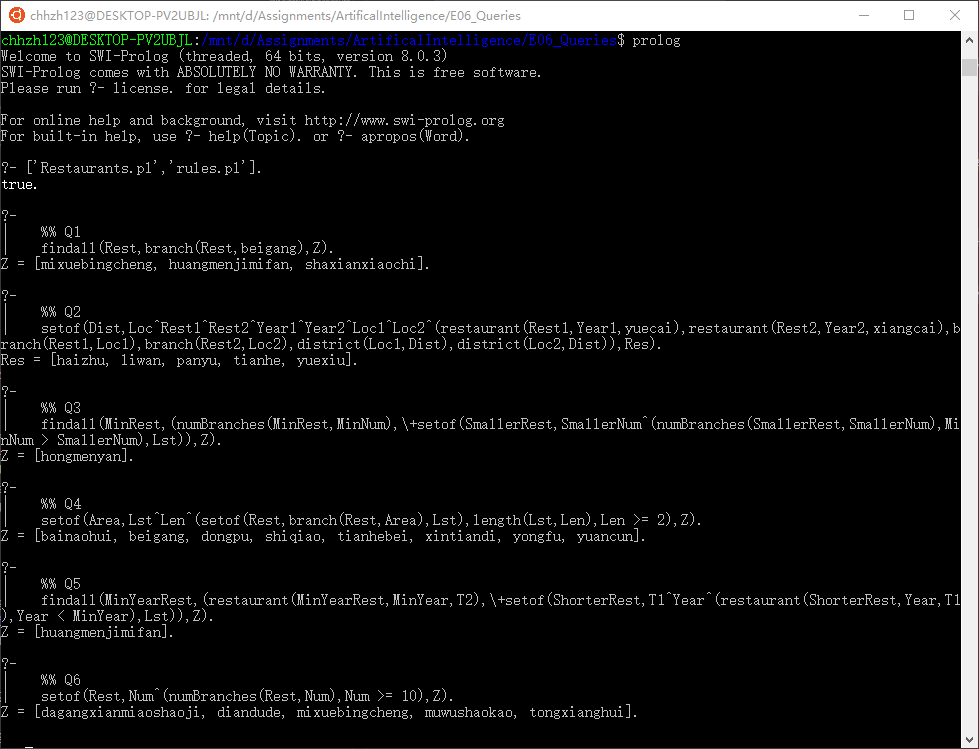
\includegraphics[width=\linewidth]{fig/results.png}
\end{figure}

I test the \verb'sameDistrict/2' rule for several cases shown below.
\begin{figure}[H]
  \centering
  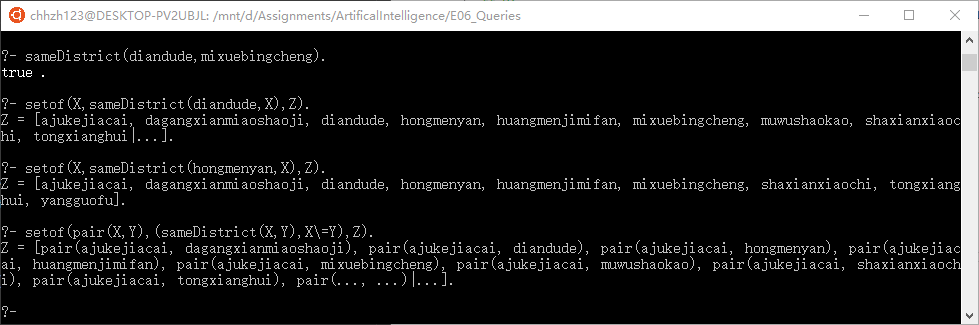
\includegraphics[width=\linewidth]{fig/results-samedistrict.png}
\end{figure}

\end{document}